
\documentclass[numbers, preprint, twocolumn,10pt]{elsarticle}

\usepackage[a4paper,margin=2cm]{geometry}

\usepackage[scaled]{helvet}
\renewcommand{\familydefault}{\sfdefault}

\bibliographystyle{elsarticle-num}
% \usepackage[numbers]{natbib}
% \bibliographystyle{abbrvnat}

%% Use the option review to obtain double line spacing
%% \documentclass[authoryear,preprint,review,12pt]{elsarticle}

%% For including figures, graphicx.sty has been loaded in
%% elsarticle.cls. If you prefer to use the old commands
%% please give \usepackage{epsfig}

%% The amssymb package provides various useful mathematical symbols
\usepackage{siunitx}
\usepackage{amssymb}
\usepackage{hyperref}
\usepackage{float}


% ---------- configure listings -------------
\usepackage{listings}
\usepackage{xcolor}
\definecolor{darkgreen}{RGB}{0,100,0}
\definecolor{darkred}{RGB}{100,0,0}

\usepackage{inconsolata}

\definecolor{codegreen}{rgb}{0,0.6,0}
\definecolor{codegray}{rgb}{0.5,0.5,0.5}
\definecolor{codepurple}{rgb}{0.58,0,0.82}
\definecolor{backcolour}{rgb}{0.95,0.95,0.92}

% ------- Unified listings setup ----------
\lstset{
    language=Python,
    backgroundcolor=\color{backcolour},
    basicstyle=\scriptsize\ttfamily,
    commentstyle=\color{codegreen}\itshape,
    keywordstyle=\color{blue},
    stringstyle=\color{codepurple},
    numberstyle=\tiny\color{codegray},
    columns=fullflexible,
    numbers=left,
    numbersep=5pt,
    xleftmargin=10pt,
    xrightmargin=5pt,
    breaklines=true,
    breakatwhitespace=true,
    showstringspaces=false,
    showspaces=false,
    showtabs=false,
    keepspaces=true,
    tabsize=2,
    captionpos=b,
    lineskip=-0.5pt,
    frame=single
}

% ========== defining instructions env ============
\usepackage{comment}
\newif\ifshowInstructions
% change to \showInstructionsfalse to hide all instructions
\showInstructionstrue
\showInstructionsfalse

\ifshowInstructions
  \newenvironment{instructions}
  {\hrule\vspace{4pt}\begingroup\color{red}\itshape}
  {\endgroup\hrule\vspace{4pt}}
\else
  \excludecomment{instructions}
\fi

%% The amsthm package provides extended theorem environments
%% \usepackage{amsthm}

%% The lineno packages adds line numbers. Start line numbering with
%% \begin{linenumbers}, end it with \end{linenumbers}. Or switch it on
%% for the whole article with \linenumbers.
%\usepackage{lineno}

\journal{SoftwareX}

\begin{document}
\renewcommand{\labelenumii}{\arabic{enumi}.\arabic{enumii}}
\onecolumn
\begin{frontmatter}
 
%% Title, authors and addresses

%% use the tnoteref command within \title for footnotes;
%% use the tnotetext command for theassociated footnote;
%% use the fnref command within \author or \address for footnotes;
%% use the fntext command for theassociated footnote;
%% use the corref command within \author for corresponding author footnotes;
%% use the cortext command for theassociated footnote;
%% use the ead command for the email address,
%% and the form \ead[url] for the home page:
%% \title{Title\tnoteref{label1}}
%% \tnotetext[label1]{}
%% \author{Name\corref{cor1}\fnref{label2}}
%% \ead{email address}
%% \ead[url]{home page}
%% \fntext[label2]{}
%% \cortext[cor1]{}
%% \address{Address\fnref{label3}}
%% \fntext[label3]{}

\title{arbok-driver: A modular and parameterized Python framework for FPGA-based quantum measurement routines}

\author[unsw]{A. Nickl\corref{cor1}}
\ead{a.nickl@unsw.edu.au}
% \ead[url]{https://github.com/andncl/arbok_drive}
\author[unsw,diraq]{A. Laucht}
\author[unsw,diraq]{A. Dzurak}
\author[unsw]{T. Tanttu}

\cortext[cor1]{Corresponding author}

\address[unsw]{School of Electrical Engineering and Telecommunications, University of New South Wales, Sydney, NSW 2052, Australia}
\address[diraq]{Diraq, Sydney, NSW, Australia}
% \address[label2]{Author2's affiliation, address, email}

\begin{abstract}
%% Text of abstract 
\textit{
    Field-programmable gate array (FPGA)-based arbitrary waveform generators are central to the control and readout of semiconductor spin qubit experiments, enabling deterministic and low-latency execution of complex pulse sequences.
    Despite the availability of high-level programming interfaces, developing scalable and maintainable measurement routines remains challenging due to the complexity of experimental logic and the large number of interdependent parameters.
    This work presents arbok-driver, a Python package that provides a dynamically generated instrument within Microsoft's QCoDeS framework for interacting with FPGA-based measurements.
    Measurement routines are defined through modular, composable and device agnostic building blocks, enabling flexible construction of complex sequences while maintaining reproducibility and scalability through device specific configurations. Relevant pulse sequence parameters are exposed to the user without requiring interaction with low-level code.
    The framework integrates with standard laboratory instrumentation, supports real-time parameter updates without recompilation, and enables adaptive measurements and feedback-based protocols.
}

\end{abstract}

\begin{keyword}
quantum measurements \sep FPGA \sep measurement framework \sep scaling qubits \sep hardware abstraction layer \sep QCoDeS \sep adaptive control
\end{keyword}

%%% This does not render correctly ...
% \begin{highlights}
% \item Dynamically generated QCoDeS instrument interface tailored to each measurement at build time.
% \item Modular, device-agnostic measurement sequences scale via declarative configurations.
% \item Synchronization loop enables live parameter updates and adaptive feedback without recompilation.
% \item Asynchronous step requirements support heralding and repeat-until-success protocols natively.
% \item Validated with \SI{300}{mm} foundry-fabricated silicon spin qubit devices.
% \end{highlights}

\end{frontmatter}

\clearpage

\section*{Highlights}
\begin{itemize}
\item Dynamically generated QCoDeS instrument interface tailored to each measurement.
\item Modular, device-agnostic sequences scale via declarative configurations.
\item Synchronization loop enables live parameter updates and adaptive feedback.
\item Asynchronous step requirements support heralding and repeat-until-success.
\item Validated with \SI{300}{mm} foundry-fabricated silicon spin qubit devices.
\end{itemize}

\section*{Metadata}
\label{}
\begin{table}[H]
    \centering
    \begin{tabular}{|l|p{6.5cm}|p{6.5cm}|}
        \hline
        \textbf{Nr.} & \textbf{Code metadata description} & \textbf{Metadata} \\
        \hline
        C1 & Current code version & v2.5.9 \\
        \hline
        C2 & Permanent link to code/repository used for this code version & \url{https://github.com/andncl/arbok_driver} \\
        \hline
        C3 & Permanent link to Reproducible Capsule & \url{https://github.com/andncl/arbok_driver/blob/master/pyproject.toml}\\
        \hline
        C4 & Legal Code License & MIT License \\
        \hline
        C5 & Code versioning system used & git\\
        \hline
        C6 & Software code languages, tools, and services used & python\\
        \hline
        C7 & Compilation requirements, operating environments \& dependencies & \url{https://github.com/andncl/arbok_driver/blob/master/pyproject.toml} \\
        \hline
        C8 & If available Link to developer documentation/manual & \url{https://github.com/andncl/arbok_driver/tree/master/docs}, \url{https://arbok-driver.readthedocs.io/en/latest/index.html} \\
        \hline
        C9 & Support email for questions & a.nickl@unsw.edu.au\\
        \hline
    \end{tabular}
    \caption{Code metadata}
    \label{codeMetadata}
\end{table}

% =============================================
\clearpage
\twocolumn

\section{Motivation and significance}
\begin{instructions}
    \textit{In this section, we want you to introduce the scientific background and the motivation for developing the software.}
    
    \begin{itemize}
        \item \textit{Explain why the software is important and describe the exact (scientific) problem(s) it solves.}
        \item \textit{Indicate in what way the software has contributed (or will contribute in the future) to the process of scientific discovery; if available, please cite a research paper using the software.}
        \item \textit{Provide a description of the experimental setting. (How does the user use the software?)}
        \item \textit{Introduce related work in literature (cite or list algorithms used, other software etc.).}
    \end{itemize}
\end{instructions}
\noindent
High-fidelity control and readout in qubit experiments place stringent requirements on the timing, synchronization, and flexibility of experimental control systems. Key operations, such as fast control pulses, coherent state manipulation via microwave or radio-frequency bursts, and time-resolved readout, require deterministic execution with minimal latency on nanosecond to microsecond timescales~\cite{jones_mid-circuit_2026, acharya_quantum_2025, bravyi_high-threshold_2024, iqbal_non-abelian_2024}. These operations must be performed within finite coherence times while maintaining high timing and amplitude precision to achieve high-fidelity control. FPGA-based arbitrary waveform generators are therefore a crucial component in many quantum platforms, enabling precise, low-latency execution of complex pulse sequences with tight multi-channel synchronization~\cite{stefanazzi_qick_2022, xu_qubic_2021, qin_fpga-based_2020}.

Programming FPGA-based control systems for quantum experiments is inherently challenging, as it requires precise handling of timing, synchronization, and low-level hardware constraints. Although most instrument manufacturers provide high-level abstraction layers that allow users to define experiments without directly writing hardware code, developing measurement routines remains difficult in practice. Experimental sequences often involve deeply nested logic, a large number of interdependent parameters, and the need to coordinate hardware-level timing with higher-level experimental workflows. As system complexity increases, maintaining flexibility, scalability, and reproducibility becomes increasingly challenging.

To address the challenges outlined above, the arbok-driver package was developed as a dynamically generated instrument driver that produces executable FPGA code from high-level Python definitions.
In a typical experimental setting, the user operates from a room-temperature control PC connected to the FPGA hardware. Measurement sequences are defined in Python by composing modular building blocks, while device-specific parameters are supplied through configuration files.
In contrast to conventional static instrument drivers, where available parameters are fixed at design time, arbok-driver constructs the instrument interface explicitly for each measurement and generates the respective sequence program in a parameterized fashion.
This allows all relevant parameters, such as wait times, voltages, and frequencies, to be automatically exposed to the user through a familiar interface, without requiring direct interaction with the generated FPGA code itself.
The workflow enables rapid iteration on experimental protocols and lowers the barrier to entry for new team members.
It supports advanced runtime features including asynchronous conditional execution and adaptive parameter streaming.
The framework has already contributed to experimental results at scale, supporting the tuning and coherent control of an eight-qubit linear array in a foundry-compatible process~\cite{nickl_eight-qubit_2025} and enabling device pre-screening that contributed to single- and two-qubit gate fidelities exceeding 99\%~\cite{steinacker_industry-compatible_2025}.

arbok-driver is integrated into QCoDeS, a Python-based framework for instrument control and data acquisition in experimental physics, developed by Microsoft's quantum computing consortium \cite{qcodes_website}.
QCoDeS provides a standardized interface for implementing and using instrument drivers, enabling arbok-driver to operate alongside other instruments within a shared measurement environment.
arbok-driver has been implemented to interface with the Quantum Machines OPX+ and OPX1000 platforms, targeting their QUA programming language~\cite{qua}. Compared to vendor-native abstraction layers such as QUAM~\cite{quam}, it integrates established instrumentation stacks via QCoDeS and supports advanced runtime features not available in those frameworks.

While a future fault-tolerant quantum computer will require embedded cryogenic control hardware\cite{patra_cryo-cmos_2018, hornibrook_cryogenic_2015, xue_cmos-based_2021}, quantum measurements on processors at the scale of tens to hundreds of qubits can still be performed using room-temperature control systems across a wide range of platforms. In this regime, flexible and scalable software abstractions remain essential regardless of the underlying qubit modality. The underlying design principles of modular sequence composition and dynamic parameter exposure are applicable to any setting in which FPGA-based control hardware is used, including superconducting qubits, trapped ions, NV centers, and quantum sensing platforms.

% ================================================
\section{Software description}

\begin{instructions}
    Describe the software. Provide enough detail to help the reader understand its impact.
\end{instructions}
\noindent
The arbok-driver framework is structured around a hierarchical composition model that separates experimental logic from hardware interaction, while remaining fully integrated within the QCoDeS instrumentation ecosystem.
A schematic overview of the architecture is shown in Fig. \ref{fig:block_diagram}.
At the top level, the ArbokDriver class acts as a QCoDeS Instrument and serves as the central interface between the user and the underlying FPGA hardware.
It operates alongside other QCoDeS compatible instruments, such as DC and AC sources, which are managed independently but coordinate with the driver within a shared measurement environment.
A Device object encapsulates the physical characteristics of the quantum device under study, providing parameter definitions that are relevant across different experiments.

\subsection{Software architecture}

\begin{instructions}
    Give a short overview of the overall software architecture; provide a pictorial overview where possible; for example, an image showing the components. If necessary, provide implementation details.
\end{instructions}

\begin{figure}[ht]
    \centering
    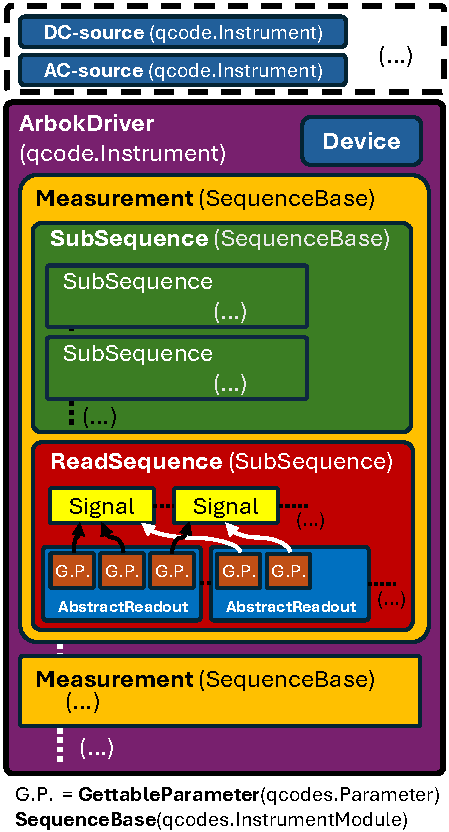
\includegraphics[width=0.4\textwidth]{arbok_block_diagram.pdf}
    \caption{
        Block diagram of the arbok-driver architecture showing the relationship between the ArbokDriver instrument, sequence hierarchy, and device configuration
    }
    \label{fig:block_diagram}
\end{figure}
\noindent
The internal structure of the ArbokDriver is composed entirely of QCoDeS InstrumentModule objects, through the SequenceBase base class.
This is a deliberate design choice, since the InstrumentModule is the native QCoDeS mechanism for organizing sub-components within an instrument, and is used in conventional static drivers to expose a fixed set of channels or functional units defined at design time.
In arbok-driver, this same mechanism is used dynamically where the sequence hierarchy is re-constructed for each measurement, reflecting the specific structure of the experimental sequence being defined.
This means that arbok-driver is not a special-purpose abstraction sitting outside the QCoDeS ecosystem, but a fully native extension of it, and all sequence components are first-class QCoDeS objects from the perspective of the framework.

The sequence hierarchy itself is built from the two classes SubSequence and Measurement which are derived from SequenceBase.
A Measurement represents a complete experimental routine and serves as the root of the hierarchy.
It is composed of one or more SubSequence objects, each encapsulating a logically distinct segment of the pulse sequence, such as an initialization stage, a control stage, or a readout.
SubSequence objects can be nested arbitrarily, allowing complex multi-stage experiments to be assembled from modular, reusable building blocks.
This recursive composition enables scalable sequence design without sacrificing readability or maintainability.

Readouts are handled by a dedicated ReadSequence class, which inherits from SubSequence and can appear at any point within a measurement, including multiple times across the hierarchy, accommodating protocols that require mid-sequence or repeated readout~\cite{jones_mid-circuit_2026}.
In practice, this means the user defines which physical signals to acquire and how they should be processed entirely through the device configuration. The same sequence code works unchanged across devices with different readout channel layouts.
Internally, a ReadSequence manages one or more Signal objects and a corresponding set of AbstractReadout instances, which are hardware-specific handlers that interface with the physical acquisition channels of the FPGA platform.
Each AbstractReadout exposes its outputs as QCoDeS Parameter objects representing measurable quantities such as demodulated quadratures or integrated voltages, allowing readout data to flow directly into the standard QCoDeS sweep and logging infrastructure.

A key design principle of arbok-driver is that the full instrument interface is generated dynamically at sequence construction time.
When a Measurement is instantiated, all tunable quantities defined across the sequence hierarchy, including wait times, pulse amplitudes, and frequencies, are automatically validated and registered as QCoDeS parameters on the ArbokDriver instrument.
Users can therefore interact with the full parameter space of a given experiment through a familiar, uniform interface, without requiring direct access to or knowledge of the underlying FPGA program.
Corresponding sequence programs are generated in a fully parameterized fashion, such that parameter updates are propagated consistently to the hardware representation.
Together, these design choices, namely hierarchical composition via native QCoDeS modules, hardware-agnostic abstractions, and dynamic parameter generation, allow arbok-driver to scale gracefully from simple single-stage sequences to the complex, multi-channel routines required in large-scale spin qubit experiments.

\subsection{Software functionalities}

\label{sec:functionalities}
\begin{instructions}
    \textit{ Present the major functionalities of the software.}
\end{instructions}

\begin{figure}[t]
\begin{lstlisting}[
    caption={Pseudo QUA program showing how arbok-driver synchronizes 
    the control hardware with the driver while making every section of the program acessible to sub-sequences},
    label={lst:qua_program},
]
# Register all QUA variables needed across the sequence hierarchy
measurement.qua_declare()

with qua.infinite_loop():
    # Pause until resumed by driver for synchronization
    qua.pause()
    # Code executed once per sweep (e.g. reset or calibration routines)
    measurement.qua_before_sweeps()
    # Nested loops over all sweep dimensions
    with qua.for_(...):
        ...
        measurement.qua_before_sequence()
        measurement.qua_sequence() # Core pulse sequence
        measurement.qua_after_sequence()

# route registered GettableParameters to hardware streaming buffers
with qua.stream_processing():
    for gettable in measurement.gettables:
        gettable.save_to_buffer()
\end{lstlisting}
\end{figure}
% At compile time, arbok-driver traverses the sequence hierarchy and constructs a QUA program, the high-level quantum programming language of the Quantum Machines platform, according to a fixed structural template illustrated in Listing.~\ref{lst:qua_program} The outermost structure of the program is an infinite loop containing a pause statement, which suspends execution at the top of each iteration until explicitly resumed by the driver. This synchronization mechanism is central to the framework's flexibility, as it allows the host computer to update instrument parameters, stream new input variables to the hardware, and trigger live data visualization between successive repetitions, without interrupting the FPGA program itself.

% Within each iteration, the Measurement exposes a set of hook methods that are delegated recursively through the full hierarchy of SubSequence and ReadSequence objects. These hooks are \texttt{declare\_variables, before\_sweeps, before\_sequence, sequence}, and \texttt{after\_sequence}, and each is invoked at a semantically distinct point in the program. This staged structure gives every component in the hierarchy the ability to place code at the appropriate location. For instance, classical arithmetic that is independent of the quantum state, such as precomputing pulse parameters, can be placed in \texttt{before\_sequence} so that it does not consume coherence time during the core pulse sequence. Finally, all GettableParameter objects registered by AbstractReadout instances across the hierarchy are automatically wired into the stream processing block of the QUA program, so that acquired data is routed to the correct hardware buffers and made available to the QCoDeS data acquisition pipeline without any additional user intervention.
\noindent
The design choices described in the previous section give rise to a measurement lifecycle with five distinct stages: build, adapt, compile, run, and interact.

\noindent
\textbf{Build.}
A measurement is constructed declaratively by composing SubSequence and ReadSequence objects into a hierarchy, either programmatically or from a nested dictionary (see Listing~\ref{lst:cpmg}). Device-specific behavior is fully determined by the configuration passed at construction time, so the same sequence definition can be reused across different devices without modification. At the end of this stage, all tunable parameters across the hierarchy are validated and registered as QCoDeS parameters on the ArbokDriver instrument.

\noindent
\textbf{Adapt.}
Before compilation, users interact with the measurement through the standard QCoDeS interface: parameters can be updated, swept, or logged without touching the underlying sequence code. Because the parameter interface is generated dynamically from the hierarchy, it always reflects the exact structure of the current measurement.

\noindent
\textbf{Compile.}
The sequence hierarchy is traversed to generate a QUA program following the fixed template shown in Listing~\ref{lst:qua_program}. Each sub-sequence places logic at semantically distinct hook points within the program, separating classical pre-computation from the timing-critical core pulse sequence. All registered GettableParameter objects are automatically wired into the stream processing block, routing acquired data to hardware buffers without additional user intervention.

\noindent
\textbf{Run.}
The compiled program executes on the FPGA within a synchronization loop that suspends execution between iterations until explicitly resumed by the driver. This loop is central to the framework's flexibility since it allows the host to update parameters, evaluate runtime conditions, and trigger data retrieval between successive repetitions without recompilation.

\noindent
\textbf{Interact.}
Between iterations, acquired data is streamed to the host for live inspection and visualization without interrupting execution. Optionally, two advanced capabilities can be configured on top of this synchronization loop. Sub-sequences can register step requirements that gate data acquisition and conditionally skip sequence sections at runtime, supporting heralding and repeat-until-success protocols. The GenericTuningInterface enables adaptive measurements by streaming new parameter values back to the FPGA between iterations, allowing optimizers or feedback algorithms to drive the measurement. Both mechanisms operate within the existing program structure and require no modification to the sequence definition.
Concrete examples of each stage are presented in Section~\ref{sec:examples}.

% ================================================
\section{Illustrative examples}

\label{sec:examples}
\begin{instructions}
    \textit{Provide at least one illustrative example to demonstrate the major
    functions of your software/code.}
    
    \textit{
        \textbf{Optional}: you may include one explanatory  video or screencast that will appear next to your article, in the right hand side panel. Please upload any video as a single supplementary file with your article. Only one MP4 formatted, with 150MB maximum size, video is possible per article. Recommended video dimensions are 640 x 480 at a maximum of 30 frames / second. Prior to submission please test and validate your .mp4 file at  \url{http://elsevier-apps.sciverse.com/GadgetVideoPodcastPlayerWeb/verification} . This tool will display your video exactly in the same way as it will appear on ScienceDirect.
        }
\end{instructions}
\noindent
The following examples demonstrate how arbok-driver is used in practice, from initial setup through increasingly complex measurement routines. Listing~\ref{lst:initial setup} shows the minimal setup required to instantiate a device and driver object. The Device object is initialised with the hardware configuration of the FPGA platform and serves as the shared reference for all subsequent measurements. The ArbokDriver object is the top-level QCoDeS instrument through which all measurements are accessed. No sequence logic is defined at this stage. All subsequent code listings in this section are intended to be executed in succession, building on this initial setup.
Measurements are independent objects that can be added or removed, or exchanged at any point without affecting the driver or any other active measurement. % could be cut out
\begin{figure}
\begin{lstlisting}[
    caption={Initializing a Device object and using it to create an empty ArbokDriver instrument},
    label={lst:initial setup},
]
from arbok_driver import ArbokDriver, Device, Measurement
from arbok_driver.examples.configurations.hardware import opx1000_config

device = Device('device_8q', opx_config = opx1000_config, divider_config = {})
my_driver = ArbokDriver('my_driver', device)
\end{lstlisting}
\end{figure}

\subsection{Scaling measurements}
\noindent
To demonstrate how arbok-driver enables scalable and reproducible measurement routines, we present the so called charge stability map as a concrete example.
A charge stability diagram is obtained by sweeping two gate voltages across a defined range and recording the resulting sensor signal at each point, mapping out the charge configuration of the quantum dot system.
It is one of the most fundamental and frequently repeated measurements in spin qubit experiments, serving both as a diagnostic tool during device tuning and as a prerequisite for qubit operation \cite{nickl_eight-qubit_2025, steinacker_industry-compatible_2025, jones_mid-circuit_2026}.
Precisely because it is so ubiquitous, it provides an ideal illustration of how a single, well-defined sequence can be deployed across devices of different scales without modification.

The same stability map routine was used in both published applications of arbok-driver.
In the two-qubit device pre-screening campaign~\cite{steinacker_industry-compatible_2025}, the measurement was executed repeatedly across multiple devices from the same 300 mm foundry process.
In this context, the value of arbok-driver lies not only in the ease of setup but in reproducibility.  Since the sequence is fully defined in code and all parameters are registered as QCoDeS parameters with explicit values, each measurement run is traceable and can be reproduced exactly on a different device or at a later date without relying on manually reconfigured instrument settings.
In the eight-qubit experiment~\cite{nickl_eight-qubit_2025}, the same routine was extended to simultaneously acquire four charge stability diagrams across all four double-dot pairs in the linear array. This required no structural changes to the sequence program itself.

\begin{figure}[]
\begin{lstlisting}[
    caption={Quantum dot electron stability map measurement creation and configuration for two and eight qubits via different configurations},
    label={lst:stability_map},
]
from arbok_driver.examples.sub_sequences import StabilityMap
from arbok_driver.examples.configurations.sequence import stability_map_8q_conf, stability_map_2q_conf

stability_meas = Measurement(my_driver, 'stability_meas')
# only change between the 2- and 8-qubit configuration:
stability_map = StabilityMap(
    stability_meas, 'stability_map', stability_map_2q_conf) # stability_map_8q_conf

detuning_range = j_range = np.arange(-0.1, 0.1, 0.01)
stability_meas.set_sweeps(
    {stability_map.v_level_P1: detuning_range,
     stability_map.v_level_P2: -detuning_range, ... },
    {stability_map.v_level_J1: j_range, ... }
)
stability_map.register_gettables( *stability_meas.available_gettables)

stability_meas.run_measurement()
\end{lstlisting}
\end{figure}

Listing~\ref{lst:stability_map} shows the measurement instantiation for both cases. The only difference between the two-qubit and eight-qubit measurement is the configuration dictionary passed at construction time on line 12. All downstream behavior, including the structure of the QUA program, the number of active readout channels, and the parameter interface exposed to the user, is determined automatically from that configuration. The sequence program for two qubits, structured according to the template in Listing~\ref{lst:qua_program}, is generated identically in both cases and can be seen in Listing \ref{lst:qua_stability_map} while the QUA output generated from the 8 qubit configuration is shown in the documentation (Tut.~1.5) \cite{arbok_docs}. 

The two different programs illustrate concretely how the framework translates a single high-level sub-sequence definition into hardware programs of different complexity, with the number of active channels, declared variables, and stream processing targets scaling automatically with the device configuration. This demonstrates that arbok-driver achieves its scalability not by requiring the user to maintain multiple versions of a sequence, but by encoding device-specific details exclusively in the configuration while keeping the experimental logic fully general.

\subsection{Defining complex measurements}
\noindent
As experimental routines grow in complexity, a measurement can quickly accumulate a large number of sub-sequences with interdependent parameters. Rather than adding these components individually, arbok-driver allows an entire sequence hierarchy to be defined through a nested dictionary, where each entry specifies a sub-sequence class, optional keyword arguments, and any further nested sub-sequences. Listing~\ref{lst:cpmg} shows this approach for a CPMG pulse sequence, a standard dynamical decoupling protocol used to characterise qubit coherence \cite{hahn_spin_1950, carr_effects_1954, naydenov_dynamical_2011}. The dictionary encodes the full structure of the measurement, from initialization through spin control to readout, and is passed to \texttt{add\_subsequences\_from\_dict} to construct the hierarchy in a single call.
For measurements that are run routinely across different devices or experimental configurations, arbok-driver provides the Experiment class as a higher-level blueprint. An Experiment object captures the invariant structure of a measurement while taking an arbitrary number of device-specific components, in this case the initialization and readout configurations, as required arguments. As shown in the lower half of Listing~\ref{lst:cpmg}, the identical CPMG measurement can be constructed from the CpmgExperiment blueprint by providing only those two components, with all internal sequence structure defined by the blueprint itself. This pattern standardizes frequently used measurements across a group or project, reducing the risk of inconsistencies between runs and making it straightforward for new users to deploy established routines on a new device.

\begin{figure}[t]
\begin{lstlisting}[
    caption={Setting up a CPMG measurement manually via a dictionary and via a pre-defined experiment},
    label={lst:cpmg},
]
from arbok_driver.examples.experiments import CpmgExperiment
from arbok_driver.examples.configurations.sequence import parity_init_conf, parity_read_conf
from arbok_driver.examples.sequences import (
    ToControlPoint, FromControlPoint,
    Xstrict, Cpmg, StateProjection
)
cpmg_conf = {
    'parity_init': {'config': parity_init_conf},
    'to_control': {'sequence': ToControlPoint},
    'spin_control':{
        'sub_sequences': {
            'x_strict': {
                'sequence': Xstrict,
                'kwargs': {
                    'target_qubit': 'Q1',
                    'control_pulse': 'control_pi2'}},
            'cpmg': {
                'sequence': Cpmg,
                'kwargs': {
                    'target_qubit': 'Q1',
                    'repetitions': 10,
                    't_equator_wait': int(1e3)}},
            'state_projection': {
                'sequence': StateProjection,
                'kwargs': {'target_qubit': 'Q1'}}},
            'kwargs':{'check_step_requirements': True}
            },
    'from_control': {'sequence': FromControlPoint},
    'parity_read': {'config': parity_read_conf}
}
cpmg_meas = Measurement(my_driver, 'cpmg_meas')
cpmg_meas.add_subsequences_from_dict(cpmg_conf)
# === or create measurement from experiment blueprint ===
cpmg_meas2 = my_driver.create_measurement_from_experiment(
    CpmgExperiment('Q1', parity_init_conf, parity_read_conf)
)
\end{lstlisting}
\end{figure}


\subsection{Asynchronous measurements}
\noindent
Measurement routines do not always follow a strictly linear execution pattern in which every repetition proceeds identically through the same sequence of steps. In many experiments it is necessary to execute certain instructions conditionally or independently of the main parameter sweep, for example to track slow drifts in qubit frequency or microwave power between sweep points~\cite{dumoulin_stuyck_silicon_2024}, or to implement repeat-until-success state initialisation protocols in which the quantum state is prepared by measurement and the sequence only continues once a desired outcome is obtained \cite{huang_high-fidelity_2024}.
arbok-driver supports this through a step requirement mechanism. Any sub-sequence can register a step requirement on its parent measurement, which is evaluated at runtime before each sequence iteration. While the step requirement is not satisfied, no data is saved to the stream processing buffers and sub-sequences that have been defined with an active step requirement, as shown by the \texttt{check\_step\_requirements} argument in Listing~\ref{lst:cpmg}, are not executed. This allows asynchronous logic such as feedback loops or heralding protocols to run continuously alongside the main sequence without requiring a separate program or manual coordination between the host and the FPGA. A comprehensive example of this functionality, including a full feedback protocol, is presented in the online tutorials (Tutorial~6)~\cite{arbok_tuts}.

\subsection{Parameter input streaming}
\noindent
So far, all examples have assumed that parameter values are defined prior to execution and remain fixed once the FPGA program is running. However, many practical optimisation problems require adaptive and non-linear exploration of parameter space, where future values depend on the outcome of previous measurements. arbok-driver supports this through a parameter input streaming interface, which allows the host computer to push new parameter values to the FPGA between sequence iterations via the synchronization loop described in Section~\ref{sec:functionalities}, without recompiling the FPGA.
The \texttt{GenericTuningInterface} builds on this feature to enable adaptive tuning workflows with minimal changes to an existing measurement definition. A parameter dictionary maps high-level tuning variables to one or more underlying QUA parameters, each with an associated scaling factor and allowed range. This makes it straightforward to couple physical parameters that must move together, such as symmetric gate voltage detuning, through a single tuning variable. Listing~\ref{lst:streaming} shows how this is applied to the CPMG measurement from Listing~\ref{lst:cpmg}, where the exchange barrier voltage and the control detuning axis are exposed as two independent tuning variables to an optimizer.

\begin{figure}[t]
\begin{lstlisting}[
    caption={Initialising a tuning interface for the CPMG measurement, 
    exposing the control detuning axis and exchange barrier as tuning variables},
    label={lst:streaming},
]
interface = cpmg_meas.initialize_tuning_interface(
    parameter_dicts = {
        'control_detuning': {
            'qua_vars': {cpmg_meas.v_control_P1: 1,
                         cpmg_meas.v_control_P2: -1},
            'bounds': (-0.05, 0.05)},
        'exchange_barrier': {
            'qua_vars': {cpmg_meas.v_control_J1: 1},
            'bounds': (0.0, 0.1)},
        },
    verbose = True
)
# interface: GenericTuningInterface
\end{lstlisting}
\end{figure}
The \texttt{control\_detuning} variable moves both plunger gates in opposite directions through a shared scaling factor, while \texttt{exchange\_barrier} controls the tunnel coupling independently. The optimizer interacts exclusively with the tuning interface and has no direct access to the underlying QUA variables or the FPGA program, keeping the adaptive logic fully decoupled from the sequence definition. A comprehensive example integrating this interface with a Bayesian optimizer is provided in the documentation (Tutorial~4)~\cite{arbok_tuts}.
% if we are not too slow we can add the pre-print of our machine leaning paper here
\section{Impact}
\begin{instructions}
\textit{
    This is the main section of the article and reviewers will weight it appropriately.
    Please indicate:
    }
\begin{itemize}
    \item \textit{Any new research questions that can be pursued as a result of your software.}
    \item \textit{In what way, and to what extent, your software improves the pursuit of existing research questions.}
    \item \textit{Any ways in which your software has changed the daily practice of its users.}
    \item \textit{How widespread the use of the software is within and outside the intended user group (downloads, number of users if your software is a service, citable publications, etc.).}
    \item \textit{How the software is being used in commercial settings and/or how it has led to the creation of spin-off companies.}
    \end{itemize}
\textit{
    Please note that points 1 and 2 are best demonstrated by references to citable publications.
    }
\end{instructions}
\noindent
The arbok-driver framework lowers the barrier to entry for engineers and researchers working with FPGA-based control systems. Since all relevant pulse sequence parameters are automatically exposed through the QCoDeS interface, new users can develop and run measurement routines without requiring direct knowledge of the underlying FPGA programming language. This is particularly valuable in growing research teams where engineers with varying levels of hardware expertise need to contribute to complex measurement workflows.

The framework has been adopted internally at Diraq, a silicon quantum computing startup, where it is currently deployed across six independent measurement campaigns spanning mass device characterisation, qubit array scale-up, benchmarking, novel qubit architectures, and automated tuning with machine learning protocols. It contributed to the tuning and coherent control of an eight-qubit linear array fabricated in a 300 mm CMOS-compatible foundry process, the largest number of qubits reported to date in this platform~\cite{nickl_eight-qubit_2025}, and supported device pre-screening from the same process, contributing to the demonstration of single- and two-qubit gate fidelities exceeding 99\%~\cite{steinacker_industry-compatible_2025}. These results demonstrate that flexible, reproducible control software is a prerequisite for translating high-fidelity qubit performance from academic settings to industry-compatible fabrication processes.

In practice, arbok-driver significantly reduces the time from setup to first measurement. New users can install the package and begin acquiring data within tens of minutes by reusing existing sub-sequences and experiment blueprints, rather than writing measurement routines from scratch. Because sequence definitions and configurations are shared across projects, measurements are guaranteed to execute identically regardless of which setup or operator runs them. Together, this accelerates the pace of research in the intermediate qubit regime by encoding experimental logic in modular, versioned Python code that facilitates systematic parameter sweeps, automated tuning routines, and the reuse of sequence components across different devices and experiments.

\section{Conclusions}
\noindent
We have presented arbok-driver, a Python package that addresses the challenge of scalable and maintainable measurement software for FPGA-based quantum control systems. The central contribution of the framework is its dynamically generated instrument interface, which constructs the full parameter space of a measurement at runtime and adapts to the specific sequence structure and device configuration of each experiment. Beyond static sequence execution, the framework supports asynchronous step requirements for conditional execution and heralding protocols, as well as parameter input streaming through the GenericTuningInterface, enabling adaptive and feedback-driven measurements without recompilation or structural changes to the underlying sequence. Standardized experiment blueprints further reduce the overhead of deploying established routines across different devices and team members. By building on native QCoDeS abstractions, the framework integrates transparently with existing laboratory infrastructure while providing a modular and fully parameterized foundation for complex pulse sequences.

The framework is particularly well suited to the intermediate scale of tens to hundreds of qubits, where room-temperature control hardware remains practical but the complexity of measurement routines demands abstractions that go beyond conventional static drivers. In this regime, arbok-driver enables reproducible, device-agnostic, and adaptable measurement workflows essential for systematic qubit characterization, automated tuning, and high-fidelity gate calibration. Currently implemented for the Quantum Machines OPX platform, a natural direction for future development is the extension of the hardware abstraction layer to support additional FPGA backends, such as Qblox's Q1ASM~\cite{qblox_q1asm}, Keysight's QCS~\cite{keysight_qcs}, or open-source alternatives like  QICK~\cite{stefanazzi_qick_2022} or QubiC~\cite{xu_qubic_2021}. Such extensions would allow the same sequence definitions and device configurations to be executed across different control platforms, further decoupling experimental logic from hardware details and broadening the applicability of the framework across the quantum computing community. % future DGX implementation 

\section*{Author contributions: CRediT}
\noindent
\textbf{Andreas Nickl}: Conceptualization, Data curation, Formal analysis, Investigation, Methodology, Resources, Software, Validation, Visualization, Writing – original draft.
\textbf{Arne Laucht}: Funding acquisition, Supervision, Writing – review and editing.
\textbf{Andrew Dzurak}: Funding acquisition, Supervision.
\textbf{Tuomo Tanttu}: Funding acquisition, Supervision, Writing – review and editing, Validation.

\section*{Acknowledgements}
\noindent
We thank E. Vahapoglu, S. Serrano, M. Candidio, S. Apicella, F. Dalmagioni, H. Vallabhapurapu and T. Botzem for user feedback and feature suggestions, and S. Bartee and A. Klopper for feedback on the manuscript. We also acknowledge P. Steinacker, W. Dumoulin Stuyck, and W. Gilbert for helpful discussions and explanations of previously used measurement techniques.

\section*{Funding sources}
\noindent
We acknowledge support from
the Australian Research Council (Grant No. FL190100167) and the U.S. Army Research Office
(W911NF-23-10092). A.N. acknowledges support from the Sydney Quantum Academy.

\section*{Competing Interests}
\noindent 
A.S.D. is chief executive officer and a director of Diraq Pty Ltd.
T.T. and A.L. declare equity interest in Diraq.
A.N. declares no competing interests.

\section*{Declaration of generative AI and AI-assisted technologies in the writing process}
\noindent
During the preparation of this work the authors used Claude (Anthropic) in order to assist with writing the software documentation, including tutorials and developer guides hosted alongside the package. The source code of arbok-driver was written entirely without AI assistance. The authors reviewed and edited all AI-assisted content and take full responsibility for the content of the published article.


\bibliography{select_references}

\clearpage
\onecolumn

\appendix

\section{QUA outputs}
\begin{figure}[H]
\begin{lstlisting}[
    caption={Output of the stability map measurement for a two qubit system defined in listing \ref{lst:stability_map}. An extended version of the measurement for 8 qubits can be found in tutorial 1 of the documentation \cite{arbok_docs}},
    label={lst:qua_stability_map},
]
from qm.qua import *
with program() as prog:
    v1 = declare(int, value=0)
    v2 = declare(fixed, )
    v3 = declare(fixed, )
    v4 = declare(fixed, )
    v5 = declare(int, )
    v6 = declare(fixed, )
    v7 = declare(fixed, )
    with infinite_loop_():
        pause()
        assign(v1, 0)
        align("P1", "J1", "P2")
        align("P1", "J1", "P2")
        play("unit_ramp"*amp(0.3), "P1")
        play("unit_ramp"*amp(-0.7), "J1")
        play("unit_ramp"*amp(0.6), "P2")
        align("P1", "J1", "P2")
        wait(12500, "P1", "J1", "P2")
        align("P1", "J1", "P2")
        assign(v4, 0.0)
        assign(v6, 0.0)
        assign(v7, 0.0)
        with for_(v5,0,(v5<20),(v5+1)):
            align()
            align("P1", "P2")
            play("unit_ramp"*amp(0.01), "P1")
            play("unit_ramp"*amp(-0.01), "P2")
            align("P1", "P2")
            align("P1", "P2", "SET1")
            wait(5000, "P1", "P2", "SET1")
            align("P1", "P2", "SET1")
            measure("measure", "SET1", integration.full("x_const", v3, ""))
            align("P1", "P2", "SET1")
            align("P1", "P2")
            play("unit_ramp"*amp(-0.01), "P1")
            play("unit_ramp"*amp(0.01), "P2")
            align("P1", "P2")
            align("P1", "P2", "SET1")
            wait(5000, "P1", "P2", "SET1")
            align("P1", "P2", "SET1")
            measure("measure", "SET1", integration.full("x_const", v2, ""))
            align("P1", "P2", "SET1")
            assign(v6, (v6+(v3*0.05)))
            assign(v7, (v7+(v2*0.05)))
        align()
        assign(v3, v6)
        assign(v2, v7)
        assign(v4, (v7-v6))
        align("P1", "P2", "SET1")
        r2 = declare_stream()
        save(v2, r2)
        r3 = declare_stream()
        save(v3, r3)
        r4 = declare_stream()
        save(v4, r4)
        align("P1", "J1", "P2")
        ramp_to_zero("P1")
        ramp_to_zero("J1")
        ramp_to_zero("P2")
        align("P1", "J1", "P2")
        align()
        assign(v1, (v1+1))
        r1 = declare_stream()
        save(v1, r1)
        align()
    with stream_processing():
        r1.buffer(1).save("qm_driver_meas_stab_2q_shots")
        r2.buffer(1).save("qm_driver_meas_stab_2q_stability_map_2q_p1p2_read")
        r3.buffer(1).save("qm_driver_meas_stab_2q_stability_map_2q_p1p2_ref")
        r4.buffer(1).save("qm_driver_meas_stab_2q_stability_map_2q_p1p2_diff")
\end{lstlisting}
\end{figure}


%% References:
%% If you have bibdatabase file and want bibtex to generate the
%% bibitems, please use
%%
%%  \bibliographystyle{elsarticle-num} 
%%  \bibliography{<your bibdatabase>}

%% else use the following coding to input the bibitems directly in the
%% TeX file.

% \begin{thebibliography}{00}

% %% \bibitem{label}
% %% Text of bibliographic item

% \bibitem{} Use this style of ordering. References in-text should also use a similar style.

% \end{thebibliography}

\begin{instructions}
\textit{
    If the software repository you used supplied a DOI or another
    Persistent IDentifier (PID), please add a reference for your software
    here. For more guidance on software citation, please see our guide for
    authors or \href{https://f1000research.com/articles/9-1257/v2}{this
      article on the essentials of software citation by FORCE 11}, of
    which Elsevier is a member.
}
\end{instructions}

\end{document}
\endinput
%%
%% End of file `SoftwareX_article_template.tex'.

%%% Local Variables:
%%% mode: latex
%%% TeX-master: t
%%% End:
